\chapter{Analiza modalna i odpowiedź układów dynamicznych} \label{sect:modal_analysis_and_response}

\textit{Streszczenie: W niniejszym rozdziale przytoczono klasyfikację metod analizy modalnej oraz przewidywania odpowiedzi dynamicznej mostów. Zaprezentowano syntetyczny opis teoretycznej analizy modalnej oraz metody wyznaczania parametrów dynamicznych konstrukcji na bazie modelu numerycznego. W dalszej części scharakteryzowano metody analityczne i numeryczne wyznaczania odpowiedzi dynamicznej modelu o jednym i wielu stopniach swobody. Na końcu rozdziału omówiono metodę uwzględniania tłumienia w analizie konstrukcji.}

\vspace{1cm}
%\section{Wiadomości wstępne} \label{section: modalAnalysisIntro}


Podstawowym celem pracy jest określenie zależności pomiędzy przyjętymi rozwiązaniami konstrukcyjnymi łukowych mostów kolejowych, a ich zachowaniem dynamicznym, a także wybór rozwiązania najlepszego. Predykcja odpowiedzi, jak wspomniano wcześniej, możliwa jest dzięki analizie numerycznym modeli MES poddanych odpowiednim obciążeniom. Jednakże trzeba zdawać sobie sprawę z niepewności, które mogą wystąpić przy konstruowaniu założeń. Rodzaje niepewności omówiono w rozdziale (\ref{sect:calibration_model}). Powiedziano również, że jedną z metod eliminacji niektórych z nich jest kalibracja modelu numerycznego. Niemniej, aby model dostosować do działania rzeczywistej konstrukcji należy mieć punkt odniesienia. Potrzebna jest więc jakaś miara zachowania statycznego lub dynamicznego obiektu. W przypadku analizy statycznej takim odniesieniem mogą być pomiary statyczne ugięć, zarejestrowane na przykład w trakcie próbnego obciążenia. W przypadku analizy dynamicznej, do porównania będą służyć charakterystyki modalne: częstotliwości i postaci drgań własnych oraz tłumienia. Parametry te można zaczerpnąć z literatury na etapie projektowania. Na etapie badania rzeczywistej konstrukcji warto zidentyfikować je w sposób eksperymentalny. W poniższym rozdziale przytoczono podstawowe zagadnienia związane z analizą modalną i identyfikacją charakterystyk modalnych układu i  obliczeniami odpowiedzi dynamicznej. Metody te zostaną w dalszej części pracy zastosowane w obliczeniach numerycznych i optymalizacyjnych.

\section{Analiza modalna} \label{section: modalAnalysisIntro}
W odpowiedzi na zapotrzebowanie przewidywania i kontroli drgań konstrukcji, w sposób naturalny rozwinęła się dziedzina nauki zajmująca się opisem i modelowaniem zjawisk dynamicznych. Podstawowym narzędziem służącym identyfikacji parametrów modalnych i testowaniu zachowania dynamicznego struktury jest analiza modalna \teng{modal analysis}. W najogólniejszym sensie analiza modalna służy określeniu częstotliwości drgań własnych oraz odpowiadających postaci i tłumień. Często analiza modalna bywa określana jako identyfikacja modalna \teng{modal identification}, a pojęcia te są traktowane zamiennie. Bywa, że niektórzy badawcze ograniczają znaczenie pojęcia analizy modalnej jedynie do wybranych metod jakie wchodzą w skład tego szerokiego pojęcia. W niniejszej pracy analizą modalną nazwane są wszystkie techniki służące poszukiwaniu parametrów modalnych konstrukcji.

W pracy \parencite{Zhang2004} autor definiuje identyfikację modalną jako gałąź szerszego pojęcia identyfikacji systemów, a jej celem jest budowa modelu matematycznego systemu dynamicznego poprzez pomiar i analizę zestawu danych wejściowych i wyjściowych. Modelem matematycznym w zagadnień dynamiki budowli jest zazwyczaj równanie lub zbiór równań, które opisują ruch modelu mechanicznego. Aby metody analizy modalnej miały zastosowanie, model matematyczny musi spełniać następujące założenia \parencite{Maia1997}:
\begin{itemize}
	\item system jest liniowy,
	\item parametry systemu są niezależne od czasu,
	\item system jest obserwowalny,
	\item obowiązuje zasada wzajemności Maxwell'a.
\end{itemize}

Ewins w  pracy \cite{Ewins2000} podaje trzy główne powody przeprowadzania analizy modalnej:
\begin{itemize}
	\item ocena źródła drgań i ich przebiegu,
	\item weryfikacja modeli teoretycznych i przewidywanie zjawisk dynamicznych,
	\item identyfikacja charakterystyk materiałowych ciała poddanego wymuszeniu dynamicznemu (np. tłumienie, tarcie, wytrzymałość zmęczeniowa). 
\end{itemize}
Każdy z powyższych celów może być jedynie środkiem do osiągnięcia zupełnie innego. W rzeczywistości tak właśnie jest najczęściej, o czym świadczy mnogość aplikacji analizy modalnej w bardzo różnych zagadnieniach dotyczących konstrukcji. 


\subsection{Klasyfikacja metod analizy modalnej}

Identyfikacja modalna jest zbiorem technik, które są rozwijane dynamicznie od lat 60' XX w. Gwałtowny przyrost zainteresowania tym tematem wywołał głównie rozwój technik cyfrowych \parencite{Ewins2000}. Do tej pory powstało wiele różnych technik, których krótką klasyfikację z podziałem na główne kryteria podano w tym podrozdziale.

Matematyczne modele modalne mogą charakteryzować się różnym stopniem skomplikowania. Jak już wspomniano, parametrami które mogą opisywać model są postaci drgań własnych oraz powiązane z nimi częstotliwości i tłumienia modalne, a także masa i sztywność modalna. Metody analizy modalnej różnią się chociażby tym, które z tych informacji mogą dostarczyć. Z tego względu wybór odpowiedniej metody powinien być świadomy i poparty przeglądem wielu technik, z których wybrana zostanie ta odpowiadająca potrzebom. Aspektami mogącymi wpłynąć na wybór metody są między innymi: czas potrzebny do implementacji (pierwszego użycia), informacje możliwe do uzyskania z modelu, możliwy wpływ założeń i uproszczeń, liczba parametrów potrzebnych do stworzenia modelu czy też stabilność rozwiązania. Podstawowe pozycje literaturowe, w których zawarto dokładny opis metod ze wskazówkami do ich użycia to \parencite{Ewins2000,Maia1997,Zhang2004,Brincker2015,Rainieri2014}. Poniżej dokonano jedynie klasyfikacji i omówienia podstawowych kryteriów podziału.

Najogólniej analizę modalną można podzielić na dwie główne gałęzie zależne od typu stosowanej procedury ogólnej, zależnej od rodzaju danych wejściowych i oczekiwanych rezultatów. Te dwie obszerne grupy nazywa się teoretyczną i eksperymentalną analizą modalną \parencite{Lengvarsky2013}. W niniejszej pracy wielokrotnie używane będą oba podejścia, dlatego autor zdecydował się na krótki ich opis. Ogólny schemat procedur teoretycznej i doświadczalnej analizy modalnej pokazano na rysunku \ref{fig:theExpProc}.  

\begin{figure}[hbt!]
	\centering
	\subfloat[Procedura teoretyczna]{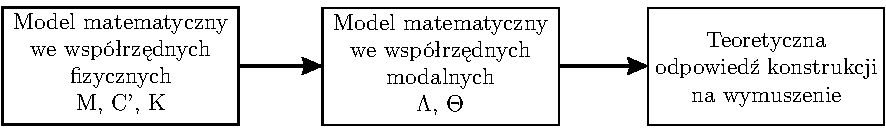
\includegraphics[width=\textwidth]{/modal_analysis/schemat_theory_exper_a.pdf}
		\label{fig:theExpProcA}
	} \\
	\subfloat[Procedura doświadczalna]{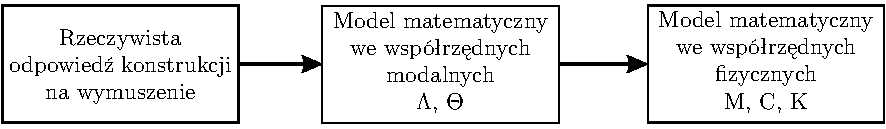
\includegraphics[width=\textwidth]{/modal_analysis/schemat_theory_exper_b.pdf}
		\label{fig:theExpProcB}}
	\captionsetup{justification=centering}
	\caption{Porównanie procedur teoretycznej i doświadczalnej analizy modalnej}
	\label{fig:theExpProc}
\end{figure}

Metody teoretyczne opierają się na rozwiązaniach analitycznych lub numerycznych (rys. \ref{fig:theExpProcA}). Badanie zachowania dynamicznego rozpoczyna się od definicji struktury, najczęściej za pomocą modelu dyskretnego opisanego macierzami $\mathbf{M}, \mathbf{C}', \mathbf{K}$, oznaczającymi odpowiednio macierz mas, tłumienia i sztywności. Na etapie dzisiejszej wiedzy, w przypadku metod teoretycznych macierz tłumienia przyjmowana jest na podstawie doświadczeń lub badań eksperymentalnych i stąd została oznaczona apostrofem $\mathbf{C'}$. Za pomocą przekształceń matematycznych tworzony jest model matematyczny we współrzędnych modalnych. Uzyskiwane są charakterystyki modalne układu $\mathbf{\Lambda}$ i $\mathbf{\Phi}$, odpowiednio częstości drgań własnych, postaci drgań własnych i dodatkowo parametry opisujące przyjęty model tłumienia. Metody analityczne znajdują realne zastosowanie w przypadku obiektów, których opis ciągły nie jest złożony, a dyskretny ograniczony jedynie do niewielkiej liczby stopni swobody. Rzeczywiste konstrukcje są układami o nieskończonej liczbie stopni swobody. Niemniej, sprowadzenie ich do skończonej (choć zazwyczaj bardzo dużej) liczby stopni swobody pozwala otrzymać zadowalająco dokładne rezultaty. W przypadku dużej liczby stopni swobody najszerzej stosowane są metody przybliżone opierające się obliczeniach numerycznych. Teoretyczna analiza modalna ma wiele zalet. Pozwala uzyskać parametry modalne relatywnie szybko i tanio. Wynika to z powszechności narzędzi do modelowania i obliczania konstrukcji. W obrębie modelowania realnych struktur współczesne oprogramowanie pozwala budować modele numeryczne praktycznie bez ograniczeń. Pomimo wielu niewątpliwych zalet, teoretyczna analiza modalna posiada ograniczenia, z których należy zdawać sobie sprawę. Przede wszystkim jakość rezultatów zależy wprost od jakości wprowadzonych przez użytkownika danych. W przypadku zagadnień dynamicznych kolejnym bardzo ważnym ograniczeniem jest brak analitycznej możliwości określenia tłumienia konstrukcji. Taką możliwość daje jedynie badanie doświadczalne. Metody analityczne i numeryczne są obszernie opisane w wielu publikacjach \parencite{Chmielewski1998,Chopra2012a,Rucka2014}. W dalszej części rozdziału zaprezentowano absolutne podstawy i założenia teoretycznej analizy modalnej.


%\cite{Brincker2015} wskazuje na następujące źródła błędów i szacowane poziomy niepewności rezultatów analizy w zależności od rodzaju popełnionego błędów w definicji modelu MES (tab):

Doświadczalna analiza w odróżnieniu od wersji teoretycznej angażuje do identyfikacji warsztat badawczy. Jak przedstawiono na rysunku (rys. \ref{fig:theExpProcB}) ten typ analizy ma niejako odwrotny kierunek niż teoretyczna analiza modalna. W tym przypadku odpowiedź konstrukcji jest mierzona i na jej podstawie wyznaczane są wielkości opisujące model matematyczny: $\mathbf{\Lambda}$ i $\mathbf{\Phi}$. Następnie dopiero na ich podstawie możliwe jest przekształcenie na model matematyczny wyrażony we współrzędnych fizycznych: $\mathbf{M}, \mathbf{C}, \mathbf{K}$. Doświadczalna analiza modalna dzieli się na dwie główne odnogi związane z zakresem rejestrowanych danych w trakcie wykonywania eksperymentu. Pierwsza z nich to Eksperymentalna Analiza Modalna (EMA) \teng{Experimental Modal Analysis}, która wymaga pomiaru sił wymuszających oraz odpowiedzi konstrukcji na to wymuszenie. Druga to Operacyjna Analiza Modalna (OMA) \teng{Operational Modal Analysis}, która estymuje parametry modalne wyłącznie na podstawie pomierzonych efektów nieznanego wymuszenia. 

Kwestia pomiaru sił wymuszających wpływa na podstawowe różnice pomiędzy EMA i OMA \cite{Bien2007}. EMA najczęściej prowadzona jest w kontrolowanych warunkach i przez to z reguły pozwala uzyskać dokładniejsze informacje na temat zachowania dynamicznego konstrukcji. Jednakże w przypadku rzeczywistych budowli trudno jest stworzyć takie kontrolowane warunki. W przypadku mostów, obiekt musiałby na czas badań zostać wyłączony z eksploatacji. Okazuje się to często niemożliwe z przyczyn proceduralnych, a do tego zawsze jest kosztowne. Drugim zasadniczym zagrożeniem powodzenia eksperymentu EMA jest potrzeba stworzenia takiego systemu wymuszenia, które wywoła mierzalną odpowiedź konstrukcji. W przypadku dużych konstrukcji inżynierskich może okazać się to trudne do zrealizowania. Oddziaływania środowiskowe często wywołują efekty porównywalne z kontrolowanym wymuszeniem. Z kolei w OMA badania prowadzone mogą być przy normalnej eksploatacji, a losowe oddziaływania środowiskowe zazwyczaj tylko polepszają jakość wyników. Niemniej jednak, teoretyczne założenia OMA prawie zawsze są spełnione jedynie w sposób przybliżony. Wpływa to na zwiększenie wymaganej długości prowadzenia pomiarów, a interpretacja wyników wymaga większego doświadczenia. 

W dalszej części tego rozdziału opisano najważniejsze - według autora - pojęcia, których zrozumienie było kluczowe do wyznaczania parametrów modalnych modelu numerycznego i odpowiedzi dynamicznej konstrukcji. Do identyfikacji modalnej istniejącej konstrukcji wykorzystano Operacyjną Analizę Modalną. Rodzinę metod OMA wraz z zastosowaniem i aplikacją przedstawiono w rozdziale \ref{sect:OMA}.

\section{Teoretyczna analiza modalna}
\label{section: eigen}
Metody teoretycznej analizy modalnej rzeczywistych konstrukcji w praktyce mają zastosowanie głównie w formie rozwiązań numerycznych prowadzonych na modelach MES. Poniżej (\ref{eq: mot_dam}) przedstawiono macierzowe równanie równowagi sił w dynamice dla tłumionego układu o skończonej liczbie stopni swobody.
\begin{equation} \label{eq: mot_dam}
\vect{M} \vect{\ddot{x}}(t) +\vect{C} \vect{\dot{x}}(t)+ \vect{Kx}(t) = \vect{F}(t)
\end{equation}
gdzie $\vect{M},\vect{C},\vect{K}$ to odpowiednio macierze mass, tłumienia i sztywności, $\vect{x}$ to wektor współrzędnych uogólnionych (przemieszczeń lub obrotów), $\vect{F}(t)$ to wektor uogólnionych sił wymuszających. Pozbawiając wzór (\ref{eq: mot_dam}) czynnika odpowiadającego za tłumienie, otrzymamy formułę (\ref{eq: mot_und}) opisującą ruch nietłumiony wymuszonego układu dynamicznego. 
\begin{equation} \label{eq: mot_und}
\vect{M} \vect{\ddot{x}}(t) +\vect{Kx}(t) = \vect{F}(t)
\end{equation}

Drgania swobodne są procesem fizycznym spowodowanym zaburzeniem stanu równowagi statycznej, przez zaistnienie niezerowych warunków początkowych. Macierzowe równanie ruchu drgań swobodnych, tłumionych opisane jest wzorem (\ref{eq: mot_dam_free}), a nietłumionych wzorem (\ref{eq: mot_und_free}). Równania te nie zawierają składnika sił wymuszających.
\begin{equation} \label{eq: mot_dam_free}
\vect{M} \vect{\ddot{x}}(t) +\vect{C} \vect{\dot{x}}(t)+ \vect{Kx}(t) = \vect{0}
\end{equation}

\begin{equation} \label{eq: mot_und_free}
\vect{M} \vect{\ddot{x}}(t) +\vect{Kx}(t) = \vect{0}
\end{equation}

Okazuje się, że parametry modalne systemu są ściśle powiązane z rozwiązaniem algebraicznego problemu własnego równań drgań swobodnych. 

\subsection{Zagadnienie własne} \label{sect:modal_analysis}
Identyfikacja modalna modelu numerycznego, polegająca na wyznaczeniu częstotliwości i postaci drgań własnych, sprowadza się do rozwiązania zagadnienia własnego. Bardzo pozytywnym aspektem tej zależności jest to, że istnieje wiele prostych w aplikacji, wydajnych i dokładnych algorytmów pozwalających rozwiązać numerycznie zagadnienie własne \parencite{Golub2013}. Dzięki temu, właśnie ta metoda identyfikacji modalnej cieszy się największą popularnością wśród producentów oprogramowania do obliczania konstrukcji. Użytkownicy oprogramowania mogą bez większego wysiłku dokonać identyfikacji parametrów modalnych nawet złożonych modeli numerycznych. Poniżej zaprezentowano zasady formułowania i właściwości zagadnienia własnego dla układu bez tłumienia (\ref{eq: mot_und_free}) i układu z tłumieniem (\ref{eq: mot_dam_free})
\subsubsection{Układ nietłumiony}
Z reguły przyjmuje się, że rozwiązanie zagadnienia własnego wykorzystuje równanie drgań swobodnych nietłumionych (\ref{eq: mot_und_free}). Należy zaznaczyć, że drgania własne nie opisują procesu fizycznego, a są jedynie matematyczną idealizacją drgań układu. W przypadku drgań własnych nietłumionym, dla każdego z modów układ oscyluje wokół położenia równowagi statycznej z częstotliwością drgań własnych, a wszystkie stopnie swobody drgają w tej samej fazie. Oznacza to, że każdy z punktów osiąga swoje ekstremalne położenie w tej samej chwili. Podobnie wszystkie punkty znajdują się w położeniu równowagi statycznej w tym samym czasie. Poniżej przedstawiono rozwiązanie zagadnienia własnego dla nietłumionego układu $N$ dynamicznych stopni swobody.

Złóżmy, że rozwiązanie równania (\ref{eq: mot_und_free}) ma postać $\vect{x}(t)=\vect{\phi}e^{j\omega t}$ gdzie $\omega$ to częstość drgań własnych, $j=\sqrt{-1}$, a $\phi$ to niezerowy wektor postaci drgań własnych. Po podstawieniu rozwiązania i jego drugiej pochodnej ($\vect{\ddot{x}}(t)=-\vect{\phi} \omega^2 e^{j\omega t}$) do równia (\ref{eq: mot_und_free}) otrzymamy równanie (\ref{eq: char_equation1}).

\begin{equation} \label{eq: char_equation1}
-\vect{M}\vect{\phi}\omega^2 e^{j\omega t} +\vect{K\phi}e^{j\omega t} = \vect{0}
\end{equation}
Dzieląc strony równania przez niezerową wartość $e^{j\omega t}$ otrzymujemy układ liniowych równań algebraicznych:
\begin{equation} \label{eq: char_equation2}
-\vect{M}\omega^2 \vect{\phi} +\vect{K\phi} = \vect{0}
\end{equation}
w którym dwie niewiadome do ustalenia to: $\phi$ - niezerowy wektor postaci drgań własnych oraz $\omega$ - częstość drgań własnych. Równanie to można zapisać w formie (\ref{eq: char_equation3}) z indeksami określającymi poszczególne mody drgań własnych. Liczba par odpowiadających sobie częstości $\omega_i$ i postaci drgań własnych $\phi_i$ jest równa liczbie $N$ stopni swobody. 
\begin{equation} \label{eq: char_equation3}
\omega^2_i \vect{M}\phi_i = \vect{K}\phi_i\qquad i=1,2,...,N
\end{equation}
Z kolei równanie (\ref{eq: char_equation4}) to reprezentacja uogólnionego problemu własnego, w którym $\lambda_i$ to wartość własna, a $u_i$ to wektor własny.  
\begin{equation} \label{eq: char_equation4}
\lambda_i \vect{A}u_i = \vect{B}u_i
\end{equation}
Z porównania wzorów (\ref{eq: char_equation3}) i (\ref{eq: char_equation4}) wyraźnie widać analogię $\lambda_i=\omega^2_i$. Wynika z tego, że rozwiązanie numeryczne uogólnionego problemu własnego pozwala wprost uzyskać częstości $(\lambda_i=\omega^2_i)$ i postaci drgań własnych $(u_i=\phi_i)$.

Układ równań (\ref{eq: char_equation3}) ma nietrywialne rozwiązania tylko, jeśli spełniona jest zależność:
\begin{equation} \label{eq: char_equation_det}
\det[\vect{K}-\omega^2_i \vect{M}] = \vect{0}
\end{equation}
Formuła (\ref{eq: char_equation_det}) jest znana jako równanie charakterystyczne zagadnienia własnego. Rozwijając wyznacznik, otrzymamy wielomian stopnia $N$ względem $\omega^2_i$. Pierwiastkami równania (\ref{eq: char_equation_det}) są częstości drgań własnych $\omega_i$. Znając częstości własne $\omega_i$, z równania (\ref{eq: char_equation3}) można obliczyć odpowiadające wektory własne $\phi_i$ z dokładnością do stałego czynnika. Taki wynik bywa nieprzystępny w ocenie więc wektory poddawane mogą być normalizacji. Do najczęściej stosowanych metod normalizacji należy taka modyfikacja wektora, aby maksymalna wartość bezwzględna spośród wszystkich współrzędnych wektora była równa jedności. Innym przykładem może być normalizacja wektorów tak, aby wartość elementu dla danego stopnia swobody, we wszystkich wektorach była równa jedności.

Jeżeli macierze $\vect{M}$ i $\vect{K}$ ($\vect{A}$ i $\vect{B}$ wg (\ref{eq: char_equation4})) są symetryczne i dodatnio określone o wartościach rzeczywistych to wartości oraz wektory własne są również rzeczywiste. W przypadku konstrukcji budowlanych macierz $\vect{K}$ jest zawsze dodatnio określona ponieważ warunki brzegowe zapewniają brak ruchu ciała jako bryły sztywnej. Nie jest to oczywiste dla innych niż struktur, takich jak na przykład samolot w locie \parencite{Chopra2012a}.


Postaci drgań własnych (wektory własne) odpowiadające różnym częstościom własnym spełniają warunki ortogonalności. W przypadku gdy $\omega_i \neq \omega_j$ prawdziwe są zależności (\ref{eq: eigenvect_orto}). Ortogonalność wektorów własnych może być wykorzystana do weryfikacji obliczonych wektorów. 
\begin{equation} \label{eq: eigenvect_orto}
\vect{\phi}_i^{T}\vect{K\phi}_j = 0 \qquad \vect{\phi}_i^{T}\vect{M\phi}_j = 0
\end{equation}

Obliczone z równania \ref{eq: char_equation_det} wartości oraz wektory własne możemy przedstawić w postaci dwóch specjalnych macierzy. $N$ obliczonych wartości własnych zestawionych w macierz diagonalną tworzy tak zwaną macierz widmową (\ref{eq: mat_spect}). Z kolei $N$ wektorów własnych zestawionych kolumnowo nazywamy macierzą modalną (\ref{eq: mat_modal}).

\begin{equation}  \label{eq: mat_spect}
\vect{\Omega}^2 =  
\begin{bmatrix} 
	\omega_{1}^2 & 0 			& \dots  & 0      \\ 
	0 		     & \omega_{2}^2 & \dots  & 0      \\
	\vdots       & \vdots       & \ddots & \vdots \\
	0 			 & 0 		    & \dots  & \omega_{N}^2 


\end{bmatrix}
\end{equation}

\begin{equation} \label{eq: mat_modal}
	\vect{\phi} = [\phi_{i,j}]= 
	\begin{bmatrix} 
		\phi_{11} & \phi_{12} & \dots & \phi_{1N} \\ 
		\phi_{12} & \phi_{22} & \dots & \phi_{2N} \\
		\vdots    & \vdots    & \ddots & \vdots \\
		\phi_{N1} & \phi_{N2} & \dots & \phi_{NN} 
	
	
	\end{bmatrix}
	\qquad
	1\leq i,j \leq N.
\end{equation}

Dla układu o $N$ stopniach swobody możemy wyznaczyć $N$ par częstotliwości i postaci drgań własnych. Jednak w rzeczywistości rozwiązanie ogranicza się do wyznaczenia jedynie ograniczonej do kilkunastu (maksymalnie kilkuset) pierwszych par. Określenie \enquote{pierwszych} właściwe jest w przypadku kiedy wyznaczone częstości uporządkujemy w szeregu rosnącym:
\begin{equation} \label{eq: eigenvalues_list}
0 \leq \omega_1  \leq \omega_2 \dots  \omega_{N-1} \leq  \omega_N
\end{equation}

W większości przypadków zagadnienie własne jest rozwiązywane numerycznie za pomocą komputerów. Metody numeryczne wykorzystują iteracyjne algorytmy do rozwiązania zagadnienia własnego. Chopra  definiuje trzy główne kategorie algorytmów \cite{Chopra2012a}: 
\begin{itemize}
	\item metody iteracji wektora wykorzystujące właściwości równania (\ref{eq: char_equation3}),
	\item metody transformacyjne korzystające z ortogonalności wektorów własnych,
	\item metody iteracyjne wykorzystujące równanie charakterystyczne (\ref{eq: char_equation_det}).
\end{itemize}
Dla dużych systemów korzystne okazuje się łączenie algorytmów z tej samej bądź różnych kategorii, co podnosi wydajność metody rozwiązania. W oprogramowaniu komercyjnym stosowane są złożone algorytmy takie jak metoda iteracji podprzestrzeni, metoda Lanczosa czy metoda gradientów Ritza. Wybór metody zależy również od wybranego solvera (silnika programu rozwiązującego równania). Algorytmy te różnią się pod względem wydajności, maksymalnej dokładności rozwiązania czy zbieżności. Ich wydajność może zależeć od liczby zadanych do wyznaczenia wartości własnych czy wielkości zadania. Więcej szczegółów odnośnie stosowanych metod rozwiązania zagadnienia własnego można odnaleźć w literaturze \parencite{Bathe2006,Wilson1983,Wilson1997,Fialko2000,Papadrakakis1993,Hughes1987,Chopra2012a}. W przypadku dobrej jakości oprogramowania komercyjnego informacje na temat używanych algorytmów powinny dostępne w dokumentacji programu.

\subsubsection{Układ tłumiony}
Drgania swobodne tłumione układu MDOF określone są równaniem (\ref{eq: mot_dam_free}), które przywołano dla wygody poniżej:
\begin{equation} \label{eq: mot_dam_free2}
\vect{M} \vect{\ddot{x}}(t) +\vect{C} \vect{\dot{x}}(t)+ \vect{Kx}(t) = \vect{0}
\end{equation}
Rozwiązanie tego równania jest uzależnione od postaci tłumienia. Może być ono klasyczne lub nieklasyczne. Tłumienie klasyczne zwane również proporcjonalnym \teng{classical damping, proportional damping} występuje w przypadku kiedy spełnione jest równanie (\ref{eq: class_damp}). 
\begin{equation} \label{eq: class_damp}
\vect{CM}^{-1}\vect{K} = \vect{KM}^{-1}\vect{C}
\end{equation}
Kiedy macierz $\vect{C}$ jest diagonalna to warunek (\ref{eq: class_damp}) jest spełniony. W takim przypadku wszystkie częstości drgań własnych są rzeczywiste i identyczne do tych wyznaczonych dla układu nietłumionego. W przypadku przeciwnym mamy do czynienia z tłumieniem nieklasycznym bądź nieproporcjonalnym \teng{nonclassical damping, nonproportional damping}. Dla tej sytuacji macierz $\vect{C}$ nie jest diagonalna, a wartości własne są zespolone. Szczegółowe informacje oraz metody rozwiązania przypadków dynamiki konstrukcji nieklasycznie tłumionych podano w \parencite{Caughey1961,Chopra2012a}. W pracy \cite{Inman1995} autorzy pokazali na przykładzie, że obliczanie struktur charakteryzujących się tłumieniem nieklasycznym za pomocą zagadnienia własnego, bez uwzględnienia macierzy tłumienia możne prowadzić do błędnych rezultatów. Tak wyznaczone częstotliwości drgań będą różnić się od rzeczywistych, co może pociągnąć za sobą błędne wnioski odnośnie zakresu częstotliwości grożących rezonansem.
\subsection{Transformacja do współrzędnych normalnych} \label{section: transform_normal}
Rozważmy ponownie równanie ruchu układu MDOF (\ref{eq: mot_dam_free2}). Wiemy, że każdy wektor o długości $N$ może być przedstawiony jako kombinacja liniowa $N$ liniowo niezależnych wektorów. Przedstawmy zatem wektor przemieszczeń $\vect{x}$ jako kombinację wektorów własnych: $\vect{\phi}$.
\begin{equation} \label{eq: normal_coord_komb}
	\vect{x} = \sum_{r=1}^{N} \vect{\phi}_r q_r=\vect{\phi q}
\end{equation} 
gdzie współczynniki $q_r$ nazywane są współrzędnymi normalnymi \teng{modal coordinates, normal coordinates} i $\vect{q}=<q_1\,\,q_2\,\, \dots\,\, q_N>^T$. Załóżmy, że zagadnienie własne zostało rozstrzygnięte i wyznaczyliśmy macierz modalną $\vect{\phi}$ (\ref{eq: mat_modal}). Aby uzyskać wartości współczynników $q_n$ dla danego $\vect{x}$, przemnóżmy obie strony równania (\ref{eq: normal_coord_komb}) przez $\vect{\phi}_n^T\vect{M}$:
\begin{equation} \label{eq: normal_coord_komb2}
	\vect{\phi}_n^T\vect{M}\vect{x} = \sum_{r=1}^{N} (\vect{\phi}_n^T\vect{M}\vect{\phi}_r) q_r
\end{equation} 

Ortogonalność wektorów własnych (\ref{eq: eigenvect_orto}) sprawia, że wszystkie składniki powyższej sumy są równe 0 poza tymi, w których $r=n$. Pomińmy więc znak sumy i zapiszmy 
\begin{equation} \label{eq: normal_coord_kom3}
	\vect{\phi}_n^T\vect{M}\vect{x} = (\vect{\phi}_n^T\vect{M}\vect{\phi}_n) q_n
\end{equation} 

\begin{equation} \label{eq: normal_coord_kom4}
	q_n = \frac{\vect{\phi}_n^T\vect{M}\vect{x}}{\vect{\phi}_n^T\vect{M}\vect{\phi}_n} 
\end{equation} 
Transformacja do współrzędnych normalnych zostanie wykorzystana przy przewidywaniu odpowiedzi wymuszonych, liniowych układów MDOF z tłumieniem proporcjonalnym (p. \ref{section: mdof_response}).

%Należy wspomnieć, że uogólniony problem własny nie jest jedyną metodą rozwiązania macierzowego równania ruchu. Przy spełnieniu powyższych warunków możliwe jest również przekształcenie uogólnionego problemu własnego w odpowiedni standardowy (prosty) problem własny:
%\begin{equation} \label{eq: eige_stan_1}
%\vect{A}u_i = \lambda_i u_i
%\end{equation}
%Aby doprowadzić równanie \ref{eq: char_equation3} do postaci standardowego problemu własnego wymagane jest wyznaczenie macierzy odwrotnej $\vect{M}^{-1}$. W przypadku kiedy jest to możliwe (na przykład przy pomocy dekompozycji Choleskiego) należy pomnożyć lewostronnie strony równania przez $\vect{M}^{-1}$ co pozwala uzyskać postać (\ref{eq: eige_stan_2}). Ponownie widoczne jest podobieństwo pomiędzy równaniami i powiązanie $(\lambda_i=\omega^2_i)$. Sprowadzenie do standardowego problemu własnego bywa korzystne z punktu widzenia rozwiązania numerycznego. 
%\begin{equation} \label{eq: eige_stan_2}
%\vect{M}^{-1}\vect{K}\phi_i=\omega^2_i\phi_i
%\end{equation}
\section{Metody wyznaczania odpowiedzi dynamicznej konstrukcji} \label{sect:dynamic_response_methods}
Wykorzystując przedstawiony w tym rozdziale opis matematyczny ruchu drgającego układów dyskretnych, poniżej zawarto metody przewidywania odpowiedzi tychże układów. W rozdziale dotyczącym efektów dynamicznych w mostach kolejowych (p. \ref{sect:railway_dynamic_effects}) wspomniano o rozwoju metod wyznaczania odpowiedzi dynamicznej pod obciążeniem ruchomym. Poniżej przywołano charakterystykę niektórych z nich. Szczególną uwagę zwrócono na metodę Newmarka, która została wielokrotnie wykorzystana w pracy. Przegląd metod pozwalających wyznaczyć odpowiedź konstrukcji poddanej wymuszeniu wypada zacząć klasycznie od układu z jednym stopniem swobody. 



\subsection{Odpowiedź systemów dynamicznych o jednym stopniu swobody} \label{section: sdof_response}

W przypadku liniowego układu SDOF obciążonego siłą zewnętrzną, równanie ruchu jest liniowym równaniem różniczkowym drugiego rzędu (\ref{eq: eq_mot_sdof}). Znając warunki początkowe $x(0)$ i $\dot{x}(0)$ możemy traktować zadanie jako w pełni sformułowane. Dla konstrukcji wstępnie nieobciążonej dynamicznie przemieszczenie i prędkość początkowe można przyjąć jako równe zeru.
\begin{equation} \label{eq: eq_mot_sdof}
	m\ddot{x}+c\dot{x}+k{x}=f(t)
\end{equation}
Dla tak sformułowanego problemu istnieją cztery podstawowe metody wyznaczenia odpowiedzi dynamicznej:
\begin{itemize}[noitemsep]
	\item klasyczne rozwiązanie równań różniczkowych,
	\item wykorzystanie całki Duhamela,
	\item rozwiązanie w dziedzinie częstotliwości,
	\item wykorzystanie metod numerycznych.
\end{itemize}
Dla porządku powyższe metody zostaną w dalszej części krótko opisane. Dokładny opis metod jest przedstawiony w podstawowych pozycjach literaturowych dotyczących dynamiki budowli \parencite{Clough1975,Chmielewski1998,Chopra2012a,Bajer2012}. 

\subsubsection{Metoda klasyczna}

Rozwiązanie liniowego równania różniczkowego o stałych współczynnikach jakim jest równanie ruchu składa się z rozwiązania całki ogólnej i szczególnej, a następnie zsumowaniu ich. Równanie ruchu jest rzędu drugiego, stąd do wyznaczenia pozostają dwie zmienne całkowania. Z kolei do ich wyznaczenia wykorzystane są warunki początkowe.

\subsubsection{Całka Duhamela}

Metoda rozwiązania równania ruchu układu SDOF za pomocą całki Duhamela polega na przekształceniu funkcji obciążenia $f(t)$ na sekwencję nieskończenie krótkich impulsów. Przykładając impulsowe, jednostkowe wymuszenie (delta Diraca) do układu (\ref{eq: eq_mot_sdof}), dla odpowiednich warunków początkowych otrzymuje się rozwiązanie w postaci odpowiedzi impulsowej, inaczej zwanej impulsową funkcją przejścia \teng{inpulse response function (IRF)}. Aby uzyskać odpowiedź układu w czasie $t$ sumuje się wszystkie odpowiedzi impulsowe do chwili czasowej $t$. W przypadku całkowalnej funkcji wymuszenia, całka Duhamela może być alternatywą do rozwiązania metodą klasyczną. Dla eksperymentalnych funkcji wymuszenia, całkę Duhamela można wyznaczyć metodami numerycznymi. W tym przypadku odpowiedź będzie wyznaczona w dyskretnych chwilach czasowych. Należy jednak wspomnieć, że w przypadku angażowania metod numerycznych całka Duhamela nie jest najwydajniejszym rozwiązaniem. Dodatkowo, ze względu na wykorzystywaną superpozycję, rozwiązanie to jest ograniczone wyłącznie do układów liniowych.

\subsubsection{Metoda przejścia do dziedziny częstotliwości}

Metoda przejścia do dziedziny częstotliwości \teng{frequency-domain method} wykorzystuje właściwości przekształceń Laplace'a lub Fourier'a. Dla układu SDOF (\ref{eq: eq_mot_sdof}) wykonuje się wybrane przekształcenie funkcji wymuszenia $f(t)$ uzyskując $F(\omega)$. $F(\omega)$ można określić jako amplitudy wszystkich składników harmonicznych, które składają się na wymuszenie $f(t)$. Przekształcenie $X(\omega)$ rozwiązania równania różniczkowego $x(t)$ można z kolei opisać następująco
\begin{equation}
	X(\omega)=H(\omega)F(\omega)
\end{equation}
gdzie $H(\omega)$ to odpowiedź zespolona w dziedzinie częstotliwości nazywana też funkcją przenoszenia lub transmitancją \teng{complex frequency-response function (FRF)}. Funkcja przenoszenia $H(\omega)$ opisuje odpowiedź układu w dziedzinie częstotliwości przy wymuszeniu harmonicznym. Ostatnim krokiem metody jest wyznaczenie rozwiązania $x(t)$ poddając $X(\omega)$ odwrotnemu przekształceniu Fourier'a bądź Laplace'a. Tak uzyskany rezultat $x(t)$ można traktować jako określenie odpowiedzi harmonicznych układu na każdy ze składników wymuszenia. Cząstkowe odpowiedzi są następnie sumowane w celu uzyskania całkowitej odpowiedzi $x(t)$. Ponownie, metoda ta bezpośrednio może być stosowana tylko dla prostych funkcji wymuszenia $f(t)$. Jeżeli funkcja wymuszenia jest określona dyskretnie, odpowiednie przekształcenia można przeprowadzić z użyciem algorytmu dyskretnej transformaty Fouriera, lub jego szybszym wariancie FFT \teng{Fast Fourier Transform}.

\subsubsection{Metody numeryczne}

Zastosowanie powyższych metod wyznaczania odpowiedzi dynamicznej ograniczone jest tylko do układów liniowych. Wspomniano również, że stają się niepraktyczne lub wręcz niemożliwe do zastosowania w przypadku skomplikowanych, zmiennych w czasie funkcji wymuszenia $f(t)$. W takich niekorzystnych okolicznościach z pomocą przychodzą metody numeryczne. Co więcej, okazuje się, że w przypadkach układów liniowych metody te są równie wydajne co metody analitycznych. 

Stworzono wiele metod i algorytmów numerycznych służących skutecznemu rozwiązaniu równań ruchu. Powstało również wiele pozycji traktujących o tym zagadnieniu \parencite{Humar1974,Hughes1987,Bathe2006,Bajer2012,Rakowski2016}. Z tego względu przytoczono tylko podstawowe pojęcia i założenia dotyczące istoty rozwiązań numerycznych.

Do rozwiązywania równań ruchu najczęściej używane są metody numeryczne oparte na bezpośrednim całkowaniu względem czasu. Bazują one na koncepcji kroku czasowego \teng{time-step} (p. \ref{section: mdof_response}). Popularność metod bezpośredniego całkowania wynika z ich uniwersalności. Należy jednak pamiętać, że nie jest to rozwiązanie ścisłe. Metody dostarczają jedynie przybliżonych rozwiązań w danych krokach czasowych, dlatego też muszą spełniać następujące kryteria:
\begin{itemize}
	\item zbieżności \teng{convergence} - wraz ze zmniejszeniem kroku czasowego, rozwiązanie powinno zmierzać do rozwiązania dokładnego,
	\item stabilności \teng{stability} - rozwiązanie powinno być stabilne pomimo występowania błędów zaokrągleń,
	\item dokładności \teng{accuracy} - rozwiązanie powinno być dostatecznie bliskie rozwiązania dokładnego.
\end{itemize}
Wśród metod numerycznych, które okazały się skuteczne w rozwiązaniach problemów dynamicznych możemy wyróżnić następujące \parencite{Rakowski2016}:
\begin{itemize}
\item uogólniona metoda różnic skończonych,
\item metoda SSPj (Zienkiewicz-Wood),
\item metoda Newmarka,
\item metoda Wilsona, 
\item metoda Houbolta.
\end{itemize}
Pomimo, że powyższe metody są opisane dla układu SDOF, są łatwo uogólniane i praktycznie wykorzystywane do obliczania układów MDOF. Algorytm metody Newmark lub podobny do niego algorytm Wilsona są najpowszechniej używane w obliczeniach konstrukcji inżynierskich.

\subsection{Odpowiedź systemów dynamicznych o skończonej liczbie stopni swobody} \label{section: mdof_response}

Systemy o skończonej liczbie stopni swobody mogą charakteryzować się tłumieniem klasycznym (proporcjonalnym) bądź nieklasycznym (nieproporcjonalnym). Mogą być liniowe lub nieliniowe geometrycznie i materiałowo. Czynniki te mają wpływ na wybór metody przewidywania odpowiedzi takiego układu. Przypomnijmy, że macierzowe równanie ruchu dla układu o $N$ stopniach swobody możemy zapisać jako $N$ równań różniczkowych w formie (\ref{eq: mot_dam})
%\begin{equation} \label{eq: mot_und_num}
%	\vect{M} \vect{\ddot{x}}(t) +\vect{C} \vect{\dot{x}}(t)+ \vect{Kx}(t) = \vect{F}(t)
%\end{equation}
 Modelem z tłumieniem proporcjonalnym, z wystarczającym przybliżeniem, można opisać większość badanych struktur. Odpowiedź układów ograniczonych do kilku stopni swobody może być wyznaczana przez rozwiązanie równania różniczkowego (\ref{eq: mot_dam}). W przypadku większej liczby stopni swobody zwykle wykorzystuje się metody numeryczne. Jak wiemy z rozdziału \ref{section: eigen}, dla takich układów zawsze możliwe jest wyznaczenie częstotliwości i postaci drgań własnych. Co więcej, opisujące je macierzowe równanie ruchu można przekształcić za pomocą metody transformacji własnej do postaci zależnej od współrzędnych modalnych. W takiej formie równanie to jest zbiorem równań rozwikłanych. Z tego względu można wyznaczyć odpowiedź dla każdego modu (zestawu jednej częstotliwości i postaci własnej oraz towarzyszącego tłumienia) osobno, a następnie złożyć je w celu wyznaczenia odpowiedzi całkowitej. Dodatkowo, każda odpowiedź modalna może być wyznaczona przez analizę układu SDOF. Te z kolei, mogą być rozwiązane wszystkimi przytoczonymi wcześniej wymienionymi metodami - w tym numerycznymi.
 
 W przypadku kiedy mamy do czynienia z układem o tłumieniu nieproporcjonalnym, klasyczne parametry modalne nie mogą być wyznaczone, a równania ruchu nie mogą być rozwikłane. Takie systemy można analizować dwiema metodami: poprzez przekształcenie równań ruchu na wektory własne obliczone w zespolonym zagadnieniu własnym lub poprzez bezpośrednie całkowanie nierozwikłanych równań różniczkowych. Druga metoda wykorzystuje metody numeryczne co wynika z braku zamkniętych rozwiązań analitycznych nawet dla analitycznie opisanych funkcji obciążenia. Metody numeryczne muszą być stosowane również w przypadku kiedy układ jest nieliniowy (niezależnie czy materiałowo, czy geometrycznie). W przypadku braku założenia o liniowości wybór metody nie jest uzależniony od tego, czy tłumienie jest proporcjonalne, czy też nie jest.
 
 Zachowując porządek i kompletność wywodu poniżej przedstawiono krótki zarys dwóch podstawowych metod wyznaczania odpowiedzi układów dyskretnych o skończonej liczbie stopni swobody.
 
 \subsubsection{Metoda superpozycji modalnej}
Rozpatrzmy układ MDOF, liniowy o tłumieniu proporcjonalnym dany równaniem (\ref{eq: mot_dam}). Wiemy, że wektor przemieszczeń $\vect{x}$ może być zapisany za pomocą współrzędnych normalnych (p. \ref{section: transform_normal}) co powtórzono dla wygody poniżej:

\begin{equation} \label{eq: superposition_modal_1_przytocz}
	\vect{x}(t) = \sum_{r=1}^{N} \vect{\phi}_r q_r(t)=\vect{\Phi q}(t)
\end{equation} 
Podstawmy \ref{eq: superposition_modal_1_przytocz} do równania (\ref{eq: mot_dam}):
\begin{equation} \label{eq: superposition_modal_2_podstaw}
	\sum_{r=1}^{N} \vect{M} \vect{\phi}_r \ddot{q}_r(t) +\sum_{r=1}^{N} \vect{C}\vect{\phi}_r \dot{q}_r(t) + \sum_{r=1}^{N} \vect{K}\vect{\phi}_r q_r(t) = \vect{F}(t)
\end{equation} 
Następnie przemnóżmy z lewej strony każdy składnik przez $\vect{\phi}_n^T$ otrzymując:
\begin{equation} \label{eq: superposition_modal_3_przemnoz}
	\sum_{r=1}^{N} \vect{\phi}_n^T \vect{M} \vect{\phi}_r \ddot{q}_r(t) +\sum_{r=1}^{N} \vect{\phi}_n^T \vect{C}\vect{\phi}_r \dot{q}_r(t) + \sum_{r=1}^{N} \vect{\phi}_n^T \vect{K}\vect{\phi}_r q_r(t) = \vect{\phi}_n^T \vect{F}(t)
\end{equation} 
Podobnie jak w punkcie \ref{section: transform_normal}, ortogonalność wektorów własnych $\vect{\phi}$ sprawia, że wszystkie składniki sum, w których $r\neq n$, zerują się. Możemy więc zapisać zredukowane równanie w postaci
\begin{equation} \label{eq: superposition_modal_4_orto}
	 (\vect{\phi}_n^T \vect{M} \vect{\phi}_n )\ddot{q}_n(t) + (\vect{\phi}_n^T \vect{C}\vect{\phi}_n) \dot{q}_n(t) + (\vect{\phi}_n^T \vect{K}\vect{\phi}_n) q_n(t) = \vect{\phi}_n^T \vect{F}(t)
\end{equation} 
Zauważmy, że iloczyny zawarte w nawiasach są skalarami. Uprośćmy więc zapis do następującej formy:
\begin{equation} \label{eq: superposition_modal_5_uprosc}
	\mathcal{M}_n\ddot{q}_n(t) + \mathcal{C}_n\dot{q}_n(t) + \mathcal{K}_n q_n(t) = \mathcal{F}_n(t)
\end{equation} 
gdzie:
\begin{equation} \label{eq: superposition_modal_6_podstawki}
	\mathcal{M}_n= \vect{\phi}_n^T \vect{M} \vect{\phi}_n \qquad 
	\mathcal{C}_n= \vect{\phi}_n^T \vect{C} \vect{\phi}_n \qquad 
	\mathcal{K}_n= \vect{\phi}_n^T \vect{K} \vect{\phi}_n \qquad
	\mathcal{F}_n(t)= \vect{\phi}_n^T \vect{F}(t)
\end{equation} 
Okazuje się, że wszystkie powyższe przekształcenia doprowadzają do tego, że (\ref{eq: superposition_modal_5_uprosc}) jest równaniem o jednym stopniu swobody dla $n$-tej współrzędnej normalnej odpowiadającej $n$-tej postaci drgań. Z tego względu współczynniki $\mathcal{M}_n,\:\mathcal{C}_n,\:\mathcal{K}_n,\:\mathcal{F}_n(t)$ nazywane są odpowiednio uogólnioną masą, uogólnionym tłumieniem, uogólnioną sztywnością i uogólnioną siłą dla $n$-tej postaci własnej \teng{generalized mass, generalized damping, generalized stiffness, generalized force}. Równanie to możemy rozwiązać wszystkimi metodami dotyczącymi układów SDOF przedstawionymi w (p. \ref{section: sdof_response}). Warto też zwrócić uwagę, że wartości $\mathcal{M}_n,\:\mathcal{C}_n,\:\mathcal{K}_n,\:\mathcal{F}_n(t)$ są uzależnione jedynie od pojedynczej postaci drgań $\vect{\phi}_n$. Naturalnie więc, jeśli znamy tylko jeden mod $\vect{\phi}_n$, możemy wyznaczyć odpowiadający mu parametr $q_n$ bez znajomości pozostałych modów.
Jeśli współczynniki normalne $q_n$ zostały wyznaczone dla $N'$ wybranych (najczęściej kilku istotnych) modów, to wkład $n$-tego modu w całkowitą wartość przemieszczeń $\vect{x}(t)$ wyznaczyć można następująco
\begin{equation} \label{eq: modal_sup_contr}
	\vect{x}_n(t) = \vect{\phi}_n q_n(t)
\end{equation}
a wykorzystując równania (\ref{eq: superposition_modal_1_przytocz}) i (\ref{eq: modal_sup_contr}) można obliczyć przemieszczenie całkowite
\begin{equation}
		\vect{x}(t) = \sum_{r=1}^{N'} \vect{x}_n(t)
\end{equation}

Sumowanie wkładu poszczególnych postaci drgań w przemieszczenie całkowite jest par excellence superpozycją. Stąd też nazwa: \enquote{metoda superpozycji modalnej}. Należy wspomnieć o paru istotnych założeniach mogących wpłynąć na wybór tej metody. Jak już wcześniej wspomniano, może być ona wykorzystana tylko w układach liniowych (ze względu na superpozycję) i tłumionych proporcjonalnie. W przypadku tłumienia nieproporcjonalnego przekształcenie równania (\ref{eq: superposition_modal_3_przemnoz}) do (\ref{eq: superposition_modal_4_orto}) nie będzie prawdziwe. Warto również pamiętać, że wynikowe przemieszczenia $\vect{x}(t)$ są niezależne od normalizacji wektorów własnych, natomiast współrzędne normalne $q_n(t)$ są od niej ściśle zależne. 

\subsubsection{Metoda całkowania bezpośredniego równań ruchu - Newmarka}
Metoda Newmarka jest algorytmem opartym na koncepcji kroku czasowego i metodach numerycznych. Zgodnie z koncepcją kroku czasowego całkowity czas podzielony jest na serię kroków czasowych $\Delta t$. Konsekwencją tego jest dyskretyzacja siły wymuszającej i odpowiedzi układu poprzez określenie ich wyłącznie w wybranych chwilach czasowych. Rozpatrzmy ponownie równanie ruchu (\ref{eq: mot_dam}):
%\begin{equation}
%	\vect{M}\vect{\ddot{x}}+\vect{C}\vect{\dot{x}}+\vect{K}\vect{x} = \vect{F}(t)
%\end{equation} 
Dokonajmy dyskretyzacji i przedstawmy siłę wymuszającą $F(t)$ określoną dla $t\in<0,t_k>$ jako zestaw dyskretnych wartości w chwilach czasowych $t_i$:
\begin{equation}
	\vect{F}_i=\vect{F}(t_i) \qquad i = 0,1,2\dots N-1,N
\end{equation}
gdzie $t_N\leq t_k$. Krokiem czasowym nazywamy różnice pomiędzy kolejnymi zdyskretyzowanymi chwilami czasowymi:
\begin{equation}
	\Delta t_i = t_{i+1}-t_i
\end{equation}
Krok czasowy jest zazwyczaj przyjmowany jako stały, ale nie jest to konieczne. Tak jak wymuszenie, odpowiedź również podlega dyskretyzacji w chwilach $t_i$, a więc równanie ruchu można zapisać w nowej formie
\begin{equation} \label{eq: motion_time_step}
	\vect{M}\vect{\ddot{x}}_i+\vect{C}\vect{\dot{x}}_i+\vect{K}\vect{x}_i = \vect{F}_i
\end{equation}
Znając warunki początkowe $\vect{x}(0)$ i $\vect{\dot{x}}(0)$ algorytmy wykorzystywane w metodach numerycznych potrafią wyznaczyć rozwiązania równania w kolejnych krokach $i = 1,2\dots N-1,N$. Należy zaznaczyć, że w metodzie \enquote{kroku czasowego} równanie ruchu nie jest spełnione w całej dziedzinie czasu, a jedynie w określonych krokiem $\Delta t$ chwilach czasowych $t_i$.

Rodzina metod numerycznych opartych na koncepcji kroku czasowego została rozwinięta przez Nathana M. Newmarka \parencite{Newmark1959}. Wykorzystuje ona dwa podstawowe równania:
\begin{subequations} \label{eq: newmark}
	\begin{align}
		\vect{\dot{x}}_{i+1} &= \vect{\dot{x}}_{i} + [(1-\gamma)\Delta t)]\vect{\ddot{x}}_{i} + (\gamma\Delta t)\vect{\ddot{x}}_{i+1} 
		\label{eq: newmark_a}\\
		\vect{x}_{i+1} &= \vect{x}_{i} + (\Delta t)\vect{\dot{x}}_{i} + [(0.5-\beta)(\Delta t)^2)]\vect{\ddot{x}}_{i}+ (\beta(\Delta t)^2)\vect{\ddot{x}}_{i+1} 
		\label{eq: newmark_b}
	\end{align}
\end{subequations}
gdzie współczynniki $\beta$ i $\gamma$ definiują zmienność przyspieszeń w trakcie kroku czasowego i istotnie wpływają na stabilność i dokładność metody. Ze względu na oba te warunki, przy braku modyfikacji algorytmu, parametry powinny mieć następujące wartości: $\gamma = \frac{1}{2}$, a $ \frac{1}{6}\leq \beta \leq \frac{1}{4}$. Na skrajach zalecanego przedziału wartości parametru $\beta$ występują dwa przypadki szczególne, w których przyspieszenie ma określony charakter w kroku czasowym:
\begin{itemize}
	\item przyspieszenie stałe - $\gamma = \frac{1}{2},\: \beta = \frac{1}{4}$
	\item przyspieszenie zmienne liniowo - $\gamma = \frac{1}{2},\: \beta = \frac{1}{6}$
\end{itemize}

Dla wartości parametrów $\gamma\ge 0.5$ i $\beta\ge0.25(\gamma+0.5)^2$ metoda Newmarka jest bezwarunkowo stabilna \parencite{Rakowski2016}. Parametr $\gamma$ odpowiada za występowanie tłumienia numerycznego, a parametr $\beta$ za stabilność metody \parencite{Bajer2012}. Wartość parametru $\gamma=0.5$ nie wprowadza żadnego tłumienia numerycznego. Przyjęcie $\beta=0$ powoduje uproszczenie równań do metody różnic centralnych.

Metoda numeryczna do wyznaczenia trzech niewiadomych $\vect{\ddot{x}}_{i+1}$, $\vect{\dot{x}}_{i+1}$ i $\vect{x}_{i+1}$ wymaga układu trzech równań macierzowych. Zatem dwa zaproponowane równania \ref{eq: newmark_a} i \ref{eq: newmark_b}, połączone z równaniem równowagi (\ref{eq: motion_time_step}) zapewnionym na końcu kroku czasowego, pozwalają wyznaczyć przemieszczenia, prędkość i przyspieszenia w chwili $t_{i+1}$. W równaniach (\ref{eq: newmark}) składniki z indeksem $i+1$ występują po obu stronach równania. Jest to tak zwana metoda niejawna \teng{implicite}, która wymaga iteracyjnego sposobu rozwiązania. Ciekawostką jest, że przyjęcie parametru $\beta=0$ modyfikuje równania w sposób, który dla układów liniowych pozwala rozwiązać układ w jednym kroku - metoda jawna \teng{explicite}. 

\section{Miary i modele tłumienia}
Drgania układów rzeczywistych zawsze są tłumione, a jedynie wielkość tłumienia decyduje o konieczności jego uwzględnienia. Wśród polskich autorów obszerne rozważania na temat tłumienia drgań mostów przeprowadził autor prac \cite{Salamak2003,Salamak2007}. Określa on tłumienie drgań w prosty sposób jako rozproszenie energii mechanicznej drgającego układu. Tłumienie można podzielić z punktu widzenia jego źródła na konstrukcyjne i zewnętrzne. Pierwsze wynika między innymi z wewnętrznego tarcia wiskotycznego materiałów w trakcie deformacji czy też niejednorodności materiału i jego spękań. Tłumieniem zewnętrznym określa się wszystkie czynniki działające z zewnątrz na konstrukcję. Mogą być związane z tarciem niechybnie występującym na łożyskach, w tłuczniu i w połączeniach, z interakcją pomiędzy konstrukcją, a powietrzem, czy z wiskoelastycznych właściwości posadowienia.

W przypadku liniowych układów zazwyczaj przyjmuje się tłumienie klasyczne, proporcjonalne opisane jak w równaniu (\ref{eq: mot_dam}). Założenie to jest powszechnie używane mimo, że na przykład wartość tłumienia jest zależna od amplitudy drgań \parencite{Ladislav1996}. Obecnie nie ma możliwości analitycznego wyznaczenia wartości tłumienia dla projektowanej konstrukcji. Niemniej istnieją opracowania, informujące o zalecanych wartościach tłumienia jakie należy przyjąć przy projektowaniu danej konstrukcji. Wynikają one z badań już istniejących obiektów. Przykładowe wartości oraz wzory empiryczne można odnaleźć w pracach \parencite{Salamak2003, Fryba1999,Bachmann2012,Yamaguchi1997}. 

W literaturze można odnaleźć kilka miar tłumienia. Pierwszą z nich jest liczba tłumienia \teng{damping ratio} nazywana również ułamkiem tłumienia lub tłumieniem względnym. Definiuje się ją jako stosunek współczynnika tłumienia wiskotycznego do tłumienia krytycznego. Dla jednego stopnia swobody (por. (\ref{eq: eq_mot_sdof})) liczę tłumienia można zapisać formułą (\ref{eq: damping_ratio_def}).
\begin{equation} \label{eq: damping_ratio_def}
	\zeta = \frac{c}{c_{kr}}=\frac{c}{2m\omega}
\end{equation}
Tłumieniem krytycznym nazywamy wartość tłumienia, po przekroczeniu której ruch staje się aperiodyczny. Dla tłumienia równego tłumieniu krytycznemu liczba tłumienia jest równa 1. W przypadku rzeczywistych mostów liczba tłumienia zazwyczaj nie przekracza 10\% \parencite{Salamak2003}. 

Inną miarą tłumienia jest Logarytmiczny Dekrement Tłumienia (LDT). Określa się go jako logarytm naturalny stosunku dwóch kolejnych amplitud drgań swobodnych danego modu:
\begin{equation} \label{eq: LDT_1}
	LDT = \ln{\frac{a_n}{a_{n+1}}}
\end{equation}
Przy małym tłumieniu wartości dwóch kolejnych amplitud mogą różnić się nieznacznie, a więc błąd powstały przy odczycie może być duży. W takim przypadku zalecane jest wyznaczenie średniego dekrementu z odleglejszych w czasie amplitud, Odczytując wartość $n$-tej amplitudy i $n+m$-tej amplitudy wartość LDT można wyznaczyć z równania:
 \begin{equation} \label{eq: LDT_N}
 	\text{LDT} = \frac{1}{m}\ln{\frac{a_n}{a_{n+m}}}
 \end{equation}
Zależność pomiędzy LDT, a liczbą tłumienia określona jest następująco:
 \begin{equation} \label{eq: LDT_dampingratio}
	\text{LDT} = \ln{\frac{q(t)}{q(t+T)}}=\ln{\frac{e^{-\zeta\omega t}}{e^{-\zeta\omega(t+T)}}} =\ln{e^{\zeta\omega T}}=\zeta\omega T = \zeta\omega\frac{2\pi}{\omega_d}=\frac{2\pi\zeta}{\sqrt{1-\zeta^2}}
\end{equation}
gdzie: $\omega_d$ - częstość drgań tłumionych $(\omega_d=\sqrt{1-\zeta^2})$, $T$ - okres drgań tłumionych $T=\frac{2\pi}{\omega_d}$. W przypadku drgań konstrukcji budowlanych liczba tłumienia jest z reguły niewielka $(\zeta<0.1)$. Z tego względu częstość drgań własnych tłumionych i nietłumionych są zbliżone. W takim przypadku zależność pomiędzy LDT, a liczbą tłumienia często upraszcza się do postaci przybliżonej:
\begin{equation}
\text{LDT} \approx 2\pi\zeta
\end{equation}

Spośród metod pozwalających na uwzględnienie tłumienia w obliczeniach najpopularniejszą jest tłumienie masowo-sztywnościowe Rayleigh'a \parencite{Chopra2012a}. Opiera się ono na stworzeniu macierzy tłumienia $\matr{C}$ bazując na liniowej kombinacji macierzy mas $\matr{M}$ i macierzy sztywności $\matr{K}$:
\begin{equation} \label{eq: rayleigh_damping}
	\matr{C}=a_0\matr{M}+a_1\matr{K}
\end{equation}
W przypadku zastosowania tłumienia Rayleigh'a liczba tłumienia odpowiadająca danemu modowi wyznaczona jest z wzoru:
\begin{equation} \label{eq: damping_rayleigh}
	\zeta_n = \frac{a_0}{2}\frac{1}{\omega_n} + \frac{a_1}{2}\omega_n
\end{equation}
Z kolei przyjmując z góry wartość liczby tłumienia można wyznaczyć wartości parametrów $a_0$ i $a_1$. Dla danych częstości drgań własnych $\omega_i$ i $\omega_j$ współczynniki Rayleigh'a wyznacza się z wzorów:
\begin{equation} \label{eq: raileigh_parameters}
	a_0 = \zeta\frac{2\omega_i\omega_j}{\omega_i+\omega_j} \qquad a_1 = \zeta\frac{2}{\omega_i+\omega_j}
\end{equation}
Wpływ składowych macierzy tłumienia pochodzących od macierzy mas i macierzy sztywności najlepiej zobrazować na przykładzie jednego stopnia swobody. Jakościowo wpływ ten przedstawiono na rysunku \ref{fig: rayleigh_chart}.
\begin{figure}[hbt!] 
	\centering
	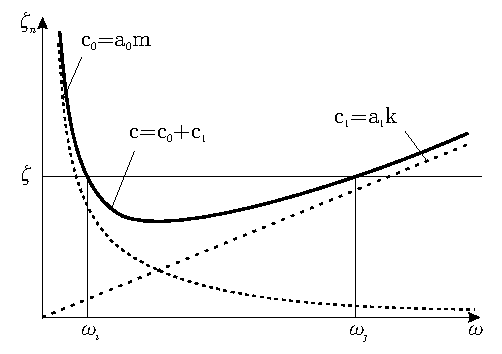
\includegraphics[]{/rayleigh/rayleigh_chart.pdf}
	\captionsetup{justification=centering}
	\caption{Wizualizacja wpływu masy i sztywności na macierz tłumienia według Rayleigh'a}
	\label{fig: rayleigh_chart}
\end{figure}
Z rysunku \ref{fig: rayleigh_chart} można wysnuć przydatne z praktycznego punktu widzenia wnioski. Założone tłumienie $\zeta$ jest spełnione jedynie dla dwóch konkretnych częstości $\omega_i$ i $\omega_j$ użytych w formułach \ref{eq: raileigh_parameters}. Składnik $c_1=a_1 k$ wzrasta liniowo wraz ze wzrostem częstości. Z kolei składnik $c_0 = a_0 m$ maleje nieliniowo wraz ze wzrostem częstości. Sumaryczna wartość obu składników dla przedziału $<\omega_i ,\omega_j>$ jest mniejsza niż zakładana. Z kolei dla częstości spoza przedziału, tłumienie jest większe niż zakładane. Jeżeli przedział interesujących częstości jest dobrany prawidłowo, to takie podejście jest bezpieczne z punktu widzenia projektanta. Jest tak ponieważ, odpowiedź modelu konstrukcji jest zawyżona względem odpowiedzi rzeczywistej struktury \parencite{Oleszek2015}.


